\documentclass[10pt,a4paper,twoside,titlepage]{report}

\usepackage[english]{babel}
\usepackage[utf8]{inputenc}
\usepackage[paper=a4paper,margin=1in]{geometry}
\usepackage[chapter]{minted}
\usepackage[hidelinks]{hyperref}
\usepackage[table]{xcolor}
\usepackage{fancyhdr,graphicx,wrapfig,booktabs,tabularx}

\graphicspath{{img/}}

\pagestyle{fancy}

\fancyhf{}
\fancyhead[RE,LO]{\rightmark}
\fancyfoot[LE,RO]{Page \thepage}

\renewcommand{\headrulewidth}{0.8pt}
\renewcommand{\footrulewidth}{0.8pt}

\fancypagestyle{plain}{
	\renewcommand{\headrulewidth}{0pt}
	\renewcommand{\footrulewidth}{0.8pt}
	\fancyhf{}
	\fancyfoot[LE,RO]{Page \thepage}
}

\definecolor{lightgray}{gray}{0.95}


\usemintedstyle{borland}

\author{Ondřej~Hlavatý, Jan~Hrach, Jaroslav~Jindrák,\\Petr~Mánek, Michal~Staruch}
\title{HelenOS USB 3.x Stack}

\begin{document}

% The title page has its special margin.
\maketitle


% Use double-sided margins from now on.
\newgeometry{top=1in,bottom=1in,right=0.5in,left=1.5in}
\cleardoublepage

% Here come the macros.

% Use these semantically, we'll improve the style later

\newcommand{\app}[1]{\texttt{#1}}
\newcommand{\lib}[1]{\texttt{#1}}
\newcommand{\struct}[1]{\mintinline{c}{#1}}
\newcommand{\fnc}[1]{\mintinline{c}{#1}}
\newcommand{\macro}[1]{\mintinline{c}{#1}}
\newcommand{\file}[1]{\href{https://github.com/helenos-xhci-team/helenos/blob/master/#1}{#1}}
\newcommand{\qemufile}[1]{\href{https://github.com/helenos-xhci-team/qemu/blob/master/#1}{#1}}


% Poor man's citations

\newcommand{\xhci}[1]{xHCI Specification, Section {#1}}


% Code environments

\newminted[bdsh]{shell}{autogobble,linenos,breaklines,frame=single,framesep=10pt}
\newminted[code]{c}{autogobble,linenos,breaklines,frame=single,framesep=10pt}




% Lists go in the front.
\tableofcontents
\newpage

\listoffigures
\newpage

\listoftables
\newpage

\listoflistings
\newpage

\cleardoublepage


% Here begins the actual content.
\chapter{Introduction}

You are reading the main documentation of the HelUSB3 project. The main goal of
the project was to extend the existing USB support in HelenOS with support for
USB 3, namely implementing the driver for host controllers compliant with the
eXtensible Host Controller Interface (xHCI), extending the USB device driver
framework to USB work at USB 3 speeds, xHCI-only devices and overall refactoring and cleanup of
the USB subsystem in HelenOS. The previous support for USB was implemented as
a software project back in 2011, then was maintained and extended by HelenOS
developers (mostly by one team member of the project).

\section{Structure of This Document}

In the first chapter, we try to build context needed to understand the
following chapters. You can get an idea of what HelenOS is and how drivers work
there. Then, we try to introduce the reader to idioms and paradigms used in the
USB world, as the rest of the documentation assumes the reader has this basic
knowledge. All of this information is included only for the sake of
completeness, we do not aim to replace (nor duplicate) the documentation of
HelenOS nor USB specifications. Please consider these sections as informative
and supportive only, and follow on topics in their respective documentations.

In the second chapter, we focus on the xHCI driver, which is a major part of
the project. We describe its overall architecture and discuss implementation
decisions. This chapter, together with in-code documentation and knowledge of the
xHCI specification, shall provide reader enough information to modify and
extend our implementation without much trouble.

The third chapter is dedicated to modifications to the existing USB subsystem.
We do not discuss the obvious ones (like support for USB 3 hubs), but those
that would be avoidable if we took the assignment to the word. Since we like to
leave the table clean, we had to change some design decisions of the previous
authors. Some of the changes introduce more systematic approach, some were
needed to implement additional parts of the assignment without using a duct
tape. Some of them are just optimizations towards better performance or
usability. Also, the documentation of the previous project was obsoletes by
recent developments in HelenOS, so we try to document the current state of
the USB subsystem.

To support the implementation process and to allow us to test it in
a semi-automatic way, we have developed a standalone testing mechanism that
tests the USB stack end-to-end by using modified virtual environment. This is
the topic of Chapter~\ref{appendix:testing}.

The last chapter concludes the documentation with a brief summary of the
accomplished project goals, instructions on how to access the materials stored
online and on the attached CD. In addition, it outlines possible future
development of the USB framework following the project end.

As the USB subsystem is mostly useless without drivers for actual USB devices,
we would like to lessen the initial barrier that stands in the way of
implementing new USB device drivers. The Appendix~\ref{chap:usb-drivers} is
written as a complete guide to writing device drivers, hiding implementation
details of the stack and focusing on how to use it only. It still requires the
reader to understand the USB architecture and mechanics though, as well as
understanding the device they are writing the driver for.

The Appendix~\ref{sec:spec} includes the official project specification (in
Czech) and a concise timeline of the project realization throughout the years
2017 and 2018.

\section{About HelenOS}
HelenOS is a microkernel operating system. Contrary to operating systems with
monolithic kernels, key operating system functionality (including device
drivers, filesystems and networking) is implemented in user-space processes (or
servers) that interact via message passing interface. The rationale of this
decision is that the failure of one component, e.g.\ a faulty driver, does not
result in the crash of the entire system. It also allows a more modular system
design.

HelenOS was started in 2004 as a software project at the Faculty of Mathematics
and Physics at Charles University and currently is being developed by students,
former students and staff of this university, among with a number of
contributors around the world. It has participated in Google Summer of Code
several times. HelenOS is used as a research operating system and as a platform
for bachelor and master theses and student software projects.

HelenOS supports several architectures (among them ia32, amd64, 32-bit ARM and
big endian MIPS) and is released under the BSD license.

\subsection{xHCI Support in Operating Systems}
\label{subsect:support-in-oses}

Extensible Host Controller Interface was first drafted in 2008 and the final
version of the specification was released in 2010. Since then, xHCI support
arrived in all mainstream operating systems like Windows, Linux, BSDs and Mac
OS X.

Regarding special-purpose, microkernel and research OSes, xHCI support is not
yet widespread.  Most notably, xHCI support is included in Google's
microkernel-based Fuchsia and in bare-metal iPXE.  Haiku Project is currently
developing xHCI driver for their OS.

In HelenOS, the support for USB was started by the HelUSB project defended in 2011. In that
time, the USB driver framework was designed, and delivered with a few USB
drivers. From the Host Controller side, UHCI and OHCI were supported almost
completely. As for the device drivers, only a generic HID driver was provided
to demonstrate the functionality of the framework. Since the project was
delivered, the USB stack evolved a little and new drivers were implemented.
The EHCI support was rather rudimentary and there was no support for xHCI.

\section{Drivers in HelenOS}

Drivers in HelenOS are separate userspace tasks. There is a common framework
for writing device drivers, the \emph{Device Driver Framework}, abbreviated as
DDF. The DDF consists of two major parts: the \texttt{devman} service taking
care about starting drivers, attaching newly found devices to drivers, and many
more; and a \lib{libdrv} library creating a platform to write DDF-compatible
drivers on.

A driver, once started, is essentially a server task. It fills a callback table
with driver operations, and waits for being called by the library. Once the
devman wants the driver to take care of a new \emph{device}, its
\fnc{dev_add} callback is called. The driver is then supposed to do whatever
it needs to make the device operating, eventually creating \emph{functions} --
nodes that are passed back to devman to be taken care of. The function can be
either an \emph{exposed} function, being a leaf node usable directly by the user
(keyboard, disk partition, \dots), or an \emph{inner} function, essentially
being a \textit{device} for another driver.

Drivers then communicate with each other using \emph{interfaces}. Every
function is provided with a set of interfaces it provides to the child driver. The
driver itself then serves as a mediator or translator of operations called on
its functions to yet another operations called on its device. For example, the
\emph{PCI} driver exposes a function for every card physically attached to the
bus. One of its functions is an xHC, which is given as a device to the
\emph{xHCI} driver. It then creates a function for every gadget connected
through USB. USB functions are provided with an interface to issue USB
transfers. USB device drivers use this interface to actually drive the USB
devices. The xHCI driver translates the transfer requests to writes into PIO
space offered by the PCI driver as a part of the PCI function interface.

In the very end, the device tree exposes only its leaves. Every leaf node
(exposed function) can be added into several categories. Categories being
a well-known classes of devices (e.g.\ a disk partition) provide an interface
of a service. For the user, the whole DDF ecosystem looks like a modular
implementation of the service interface, allowing them, for example, to mount
the partition regardless of where it is located and how it is connected to the
system.

\section{Briefly about USB}
\label{sec:usb_briefly}

Disclaimer: This chapter is heavily copied from the documentation of the
previous project \textit{USB subsystem in HelenOS} and filled in with the new
features and specifics of USB 3.

This chapter provides a brief overview of the USB architecture. It does not aim
to be a drop-in replacement for Universal Serial Bus specifications. It can be
also viewed as a summary of what the reader of this document must already know.
If you are new to USB, you can use this chapter as a starting point for further
reading.

\subsection{The ‘big’ picture}

USB is a technology used for connecting peripherals to host computer. Its main
advantages are simplicity of usage for end users, pretty good scalability (in
terms of number of simultaneously attached devices) and a choice of possible
transfer types that accommodate requests of diametrically different devices.
The USB defines the following aspects (most of them will be mentioned later in
this chapter):

\begin{itemize}
\item bus physical topology
\item physical interface — both mechanical (plugs) and electrical
\item power management
\item configuration of attached devices
\item querying attached devices for supported functions
\item low-level data protocol used on the bus
\item high-level data protocol — transfer types
\end{itemize}

The following sections will describe parts that are most important for
programmers of USB related software, such as device drivers or host
controllers. They will not include description of low-level aspects, such as
electrical current settings or sizes of mechanical plugs. The acronym USB is
used in two slightly different meanings in the following text. First, as a
common prefix (e.g. USB device), second in its original meaning, describing the
bus itself (when the word ‘bus’ is used, it will always refer to the Universal
Serial Bus unless explicitly stated otherwise).

\subsection{Bus topology}

USB uses a tree-like physical bus topology. In the root of the tree there is
the host computer with a hardware chip — host controller — controlling all
communication over the bus. All communication requests of device drivers are
directed to the driver of the host controller that schedules them and then
sends them to the USB ‘wire’. The host controller provides several
\textit{ports} to which devices are connected.

USB devices come in two flavors. First, there are \textit{functions} — these
provide actual functionality and create leaf nodes in the bus topology. An
example of an USB function is a printer or a keyboard. The other kind are
\textit{hubs} that create branches on the bus and to which the other devices
might be connected.

Hubs provide means to attach more devices to the same bus. The attachment place
is called a port (typical hubs for PCs has about four ports). Each hub has two
different kinds of ports. First, there is the upstream port through which the
hub is connected to a parent device (i.e. the predecessor in the tree) and then
there are several downstream ports through which the other devices are
connected. The host controller must always provide at least one port to allow
device attachment. Typically, the ports provided by the host controller are
provided by its own hub, called \textit{root hub}.

Although physically, the topology is a tree rooted in the host controller,
device addressing uses a flat structure and under certain abstraction, hubs can
be viewed as transparent splitters that add no logic to the bus.

Each device connected to a host controller receives an unique address (a
positive integer) and reacts only to communication that is targeted to it.
Before the device receives this address, it listens on the \textit{default
address} (number zero). To prevent situation when more devices would listen on
the default address simultaneously, each hub must provide means to disable
communication forwarding to certain ports (USB terminology says that hub does
not \textit{signal} on given downstream port).

\subsection{Device configurations, interfaces and endpoints}

USB was designed to be as flexible regarding device configurations as possible.
Because of this, each device can provide several \textit{configurations}. Each
configuration may provide completely different sets of features but in reality
practically almost all common USB devices have only a single configuration.

Each configuration can provide one or more \textit{interfaces}. The interface
provides the actual functionality of the device. For example, an USB printer
provides the printing as an interface. Some devices may provide multiple
interfaces. For example, a digital camera may provide an interface for direct
communication with the camera (usually via vendor-specific drivers) and, as a
fallback, a mass-storage interface that can be used to download photos when the
specialized drivers are not available.

Each interface can have several \textit{alternate settings} that change device
capabilities at the interface level. For example, network card may offer
several alternate settings using different sizes of data packets, or cameras
offering an alternate setting for each supported resolution.

The actual communication with the device performed through \textit{endpoints}.
Each endpoint belongs to a single interface and represents a communication
‘gate’ to the device — USB uses the term \textit{pipe} to describe an abstract
connection between the device driver on one side and the device on the other
one. Endpoints are usually unidirectional (exceptions are control endpoints)
and they have several attributes that must be obeyed by the driver.

A special endpoint — \textit{control endpoint zero} (also called default
control endpoint) — is present on each device and is used for configuration
purposes and for standard requests (e.g. for querying the device for
generic capabilities).

\subsection{Bus protocol and transfer types}

The USB defines how data that are supposed to be sent to (or received from) a
device shall be encoded and treated prior to their sending over the wire. This
overview skips the physical aspect of the communication and starts with an
abstraction, that the host controller has, which is a way to send a stream of
bytes using the wire.

Communication over the bus uses data \textit{packets} which encapsulate the
actual payload and some service data. The service data include target address,
endpoint number, packet type and data needed for packet integrity checks.

Before moving on to describing packet types, it is necessary to mention
transfer types. In order to allow devices with different transfer requirements
(e.g. web camera that supplies a continuous stream of data vs. keyboard with
few bytes several times minute) the transfers (and therefore endpoints) are
divided into four different types.

The first type of transfers are \textit{control transfers}. These are used for
the device configuration and for manipulating the state of the device. Every
device has at least the default control endpoint but it is possible for the
device to have multiple control endpoints. The control transfers are
bidirectional.

The second type are \textit{interrupt transfers}. These are intended for small
and infrequent data where minimizing the latency is the primary goal. These are
considered periodic transfers and the host controller reserves a part of the
bus bandwidth for them. The typical devices using this transfer type are all
HID devices.

The third type of transfers are \textit{bulk transfers}. Bulk transfers are
used to send large chunks of data over the bus when the requirements are to
have correct data and no requirements on the delay is acceptable. Typical
devices include printers, scanners or external disks. USB 3 also introduces
streams as an another layer of abstraction over bulk transfers.

The last type of transfers are \textit{isochronous transfers}. Unlike bulk
transfers, where data integrity is a priority, isochronous transfers ignore
data integrity and all priority is put on quick and periodic delivery (policy
is that delayed data are worse than damaged ones). Multimedia devices such as
web-cameras or wireless controllers use this transfer type.

When a device driver wants to send data to the device (the device cannot
initiate the transfer), it gives the payload to the host controller together
with information about target device (address) and endpoint. It must also
provide information about transfer type and data direction. For incoming
transfers, it instead reserves the data buffers to which the device can send
the data. The host controller then encapsulates these information. In case of
USB 2, it creates three packets. The first packet informs about data direction
and it's called the token packet. The second packet transfers the actual data.
The last packet is a handshake packet and it is used to acknowledge the
transaction. In case of USB 3, the same parts are used differently. For
outgoing transactions, the token is incorporated in the data packet; while for
ingoing transactions, the token is replaced by a handshake.

This protocol is roughly the same for bulk, interrupt and isochronous
transfers. Control transfers are a bit different because they have a special
preamble — a setup packet. The setup packet contains commands that might
change the device state and this packet might be optionally followed by a data
phase. The control transfers are the only ones that are actually bidirectional
(because the setup packet is always outgoing, while the data phase could be
either in or out).

\subsection{Device descriptors and device classes}

In previous sections querying USB device for its capabilities was mentioned.
This sections will describe this querying in more detail. Each USB device must
provide several data blocks, called \textit{descriptors}, describing its
configuration and capabilities. Some descriptors are device dependent while
others are generic for any USB device.

The roughest description of a device is provided in a \textit{device
descriptor}. It holds information about device vendor, device class (see
below), number of possible configurations and several other details.

Each configuration is then described by a \textit{configuration descriptor}.
This descriptor also contains the number of interfaces the configuration
provides. Each interface is then described by an interface descriptor. The
interface descriptor specifies to which class the interface belongs and how
many endpoints it specifies.

Unsurprisingly, each endpoint is described by an \textit{endpoint descriptor}.
This descriptor defines attributes of the endpoint — data direction, transfer
type and endpoint number.

In case of USB 3, an endpoint descriptor is followed by a \textit{superspeed
endpoint companion descriptor}. This defines USB 3 specific features such as
burst transfer support or bulk streams.

The descriptors can be viewed as a tree, where the device descriptor is the
root node that has several descendants — configurations. Each configuration
then groups interfaces and endpoint descriptors are leaves. Device may provide
its own descriptors (e.g. vendor specific ones) that may stand aside of this
tree or be part of it (then they are typically inserted somewhere between
interfaces or endpoints).

Although logically the descriptors form a tree, the device usually returns them
in a serialized manner. For example, interface and endpoint descriptors can be
retrieved only as a part of a configuration descriptor they belong to. The
ordering in the serialized form implies the logical tree it represents.

USB was designed with flexibility of offered functionality in mind but to
prevent total chaos, devices (or rather their functionality) were divided by
common attributes into so called \textit{device classes}. Each class deals with
devices of certain kind, e.g. HID devices, printers, scanners, audio or a
special vendor class for any device that would not fit into any other one. Some
classes define \textit{subclasses} for fine-grained resolution (e.g. HID class
offers subclass for keyboards and mice).

The class is reported as a part of device and interface descriptor. That is
because a single physical device may provide functionality of several classes
simultaneously, depending which interface the software communicates with. In
such cases the class reported through the device descriptor is a special value
with meaning ‘no class, see interface’.

\subsection{Bus enumeration}

USB was designed with possibility of hot-plugging and thus it has to have well
defined actions when a new device is added. The following is a simplified
sequence of what all the involved drivers and devices must go through. The
setup is that new device is attached to some hub, that is already initialized
and configured.

\begin{enumerate}
\item The hub (the hardware) detects change on one of its ports.
\item The hub waits some time to allow electrical current stabilization.
\item The hub informs the driver that a change occurred.
\item The hub driver queries the hub for exact kind of change (whether device
was added or removed, etc.).
\item The hub driver requests reservation of default address (to prevent having
more devices listening on the same address).
\item The hub driver tells the hub to enable the port.
\item The port is enabled (i. e. signaling is open), the driver then must wait
again for stabilization of currents.
\item The driver queries the device for its device descriptor and assigns a new
address to it.
\item The driver can release the reservation of the default address.
\item Based on the values of device descriptor, proper driver for the new
device is found and started.
\end{enumerate}

The new driver is then told the address of the device and it is up to it to
configure and finish the initialization of the device.
As stated above, the sequence is simplified and due to errors in devices (not
all USB devices obey the specification exactly) some steps (e.g. setting new
address) have to be tried several times or in specific ordering.

\subsection{USB communication}

\subsubsection{Packets, transactions, transfers}

The communication on USB bus is \textit{packet} oriented. Every piece of
information sent to device or host is translated into packet form before it
reaches the bus.

However, packet level is not accessible to the software and drivers are not
able to sent separate packets. The smallest communication entity available is
called a \textit{transaction}. These differ between various USB version and
therefore won't be described here. See USB specifications for different
transaction types of each USB version.

Requests handled by host controller drivers are called \textit{transfers}. One
transfer usually corresponds to one command to the device. Transfers may
consists of several transactions. USB specification distinguishes the four
types of transfers already described above: control transfers, interrupt
transfers, bulk transfers and isochronous transfers.

These transfers have their specifics which are not exposed by the xHC.
Therefore, the only transfer type requiring special behavior is control
transfer type.

Control transfers consist of three stages:
\begin{itemize}
\item \textbf{SETUP stage}: uses setup transaction and identifies command to
the device
\item \textbf{DATA stage}: optional, the direction (IN/OUT) and its presence
depends on the command sent in setup stage
\item \textbf{STATUS stage}: direction used in STATUS stage is opposite to that
in DATA stage. If data stage was not present direction of STATUS stage is IN.
\end{itemize}

Control transfers must complete all stages without being interrupted by another
control transfer to the same endpoint. If two or more control transfers
interleave, it will result in failure of the interrupted transfers.

\subsubsection{Bus access constraints}

Different transfer types have different bus access limitations. Periodic
transfers (isochronous and interrupt),are limited to 90\% of the available
bandwidth. Interrupt and isochronous communication happens regularly (hence
periodic) and maximum requested bandwidth has to be reserved in advance.
Failure to reserve the bandwidth results in an error. The driver may then
choose another interface setting or it can report an initialization failure.

At least 10\% of bandwidth has to be available for control transfers. It might
be less if there are not enough control transfers pending.

Bandwidth, that is left unused after periodic and control transfers requests
were satisfied is used by bulk transfers. Bulk transfers work in best effort
mode and if there is no available bandwidth they are postponed.

It is the role of host controller driver scheduler to guarantee bus access
constraints.

\subsection{USB 3 features}

\subsubsection{Bus duality}

The USB 3 bus and USB 3 devices are backwards compatible with USB 2. As the
protocol is completely different this was done by splitting the bus into two
parts. The physical implementation is best shown by the following figure.

% TODO Reference this figure to the USB 3 specification, section 3.1, fig 3-1

\begin{figure}[h]
	\centering
	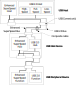
\includegraphics[width=0.6\textwidth]{dual-bus}
	\caption{Dual bus architecture}
	\label{fig:dual-bus}
\end{figure}

Every USB 3 device can be seen as both USB 3 and USB 2 device. If an USB 3
device is plugged into USB 2 hub, the device will recognize that and start
communicating using its USB 2 hub and exposing only USB 2 function.

If on the other hand a USB 3 device is plugged into USB 2 hub (that is plugged
into USB 3 compatible host controller), the device cannot communicate using USB
3 bus as the parent hub doesn't support it.

The specification doesn't require the device to have the same function in both
USB 2 and USB 3 modes. For example, the USB 2 function may be used to only
describe that the device can only operate in USB 3 mode.

\subsubsection{Differences from USB 2}

USB 3 introduces several new features used to speed up the communication and
offer more bandwidth. Most of these features are hidden to the device drivers.
They will be described in this section.

One of the new features USB 3 introduces is called bursting. An endpoint that
supports bursting states its maximum data burst size in its SuperSpeed Endpoint
Companion descriptor. When a transfer is initiated the sender may send multiple
packets in a row before it has to wait for an explicit handshake. This
eliminates the wait time and improves the communication efficiency.

Unlike USB 2 and previous version where the bus was half-duplex, the bus in USB
3 is full duplex. This means that a device using USB 3 may use both IN and OUT
transactions concurrently.

The devices on USB 2 bus communicate using broadcast. For OUT transactions,
every hub broadcasts the packet to all enabled downstream ports and only the
targeted device should accept the packet. In USB 3, the communication is
routed directly to the receiver. This introduces the need for route strings,
which describe the ports of the hubs on the way to the device.

In USB 2, the drivers are required to use polling as a way to find out that the
transfer has finished. USB 3 introduces asynchronous notifications to reduce
the overhead and simplify the driver design.

At last but not the least, USB 3 introduces more complex power management
features. For example, an USB 3 device may initiate link power state change at
the device while in USB 2, this could be only initiated by the host.


\section{Existing USB Subsystem}

As mentioned in subsection~\ref{subsect:support-in-oses}, HelenOS already supported
UHCI, OHCI and to some extent EHCI.

The original documentation of the HelUSB project described the state of affairs
as the project ended. Since then, several improvements in both USB support
and in HelenOS driver framework in general were made, for example new USB
drivers like mass-storage were added. Unfortunately, these changes are pretty
much not documented anywhere. In this section, we will focus on the things that changed since the
documentation was written. We do not aim to replace the original documentation
of HelUSB project.

\vspace{1.5em}
\textsl{By all means, information in this chapter is written with
regard to the state before \emph{our} project was implemented. Thus, great part
of the information given in this section is already obsolete, but it's needed to
assess the damage we're personally responsible for.}
\vspace{1.5em}

The USB framework defines two classes of drivers -- the host controller drivers
and USB function drivers. For the first class, there is a library called
\lib{libusbhost} that aids in providing the unified interface of the host
controller to USB function drivers, and also implements common HC
functionality. There are four HC drivers at the moment:

\begin{itemize}
\item
	\textbf{VHC}, Virtual Host Controller. Implemented in the early phase of
	HelUSB project, served probably as a dummy backend to allow better work
	parallelization and debugging.

\item
	\textbf{UHCI}, Universal Host Controller Interface driver. The earliest
	interface supporting speeds of USB 1.0: Low- and Full-speed devices.
	Important for running HelenOS under QEMU, as it's the interface of the
	default HC QEMU emulates. Apart from isochronous transfers, the driver
	covers all functionality UHCI provides.

\item
	\textbf{OHCI}, Open Host Controller Interface driver. Somewhat complete,
	yet a bit simplified, especially in terms of transfer scheduling. Does not
	care about the polling interval, but schedules all interrupt transfers on
	every frame. Isochronous transfers not supported.

\item
	\textbf{EHCI}, Enhanced Host Controller Interface driver. Mostly a copy of
	OHCI driver, as it uses similar structures. Shall support USB 2 speeds, but
	the support is very limited -- the driver cannot use High-speed hubs to
	communicate with Full- and Low-speed devices, as the support for
	Transaction Translation is completely broken. Also, the bandwidth
	accounting is not implemented for High speed. Neither this controller
	supports isochronous transfers.
\end{itemize}

The HC driver is no longer split in half (as the project documentation states),
but all HC drivers emulate a virtual hub that is driven by a regular
\lib{usbhub} driver. The tree physical topology of USB is kept only inside the
HC driver, and is presented flat to the Device Driver Framework -- all USB
devices are child functions of the HC driver. They communicate with each other
through the DDF driver interface called \texttt{usb\_iface}, which contains all
methods various drivers use.

When the driver enumerates a USB function, it is usually taken care of by the
\lib{usbmid} driver. This driver scans the device descriptor for provided
interfaces, and creates child functions for them. These functions are then
driven by class drivers. Notable exception being the \lib{usbhub} driver,
taking care of the device directly, as hubs are not allowed to have multiple
interfaces.

The USB function drivers are well supported by the \lib{libusbdev} library.
This library builds an abstraction layer above \lib{libdrv}, used by other
drivers directly, to better suit the needs of USB devices. It does a complete
initialization of the USB device, including initiating a separate IPC
connection to the HC driver directly -- to avoid bouncing all operations in the
\lib{usbmid} driver. For this purpose, the \texttt{usb\_iface} contains two
methods: \fnc{get_my_iface} and \fnc{get_my_interface_handle}. The first one is
answered by the \lib{usbmid} driver with the number of interface driven, or
with a value of $-1$ by the HC driver if the driver serves the whole device.
The \fnc{get_my_interface_handle} call is recursive, until it reaches the HC
driver -- which answers it with devman handle of the USB device function. The
device driver then uses it to initiate connection to the HC driver, the same
way as the usbmid driver does.

Although this is sort-of hacky solution (the devman handle is supposed to be
private), it is currently the only one. Ideally, the drivers would use
a special method to let new connection forward to the HC driver, but for
complicated reasons, this does not work as expected. We discussed this with the
current HelenOS developers, and they confirmed us that the issue is still not
solved.

The \lib{usbhub} driver uses another four methods defined by the
\texttt{usb\_iface}. The interface methods \fnc{reserve_default_address} and
\fnc{release_default_address} ensure synchronization across multiple hubs
(possibly across multiple hub drivers), as the software must ensure that only one
device is listening on the default address at the same time. Then,
\fnc{device_enumerate} and \fnc{device_remove} announce that a device is
connected to (detached from) the hub, to be enumerated (removed) by the HC
driver. The interesting part is that the hub driver has no access to the
created device, as the logical topology presented to the DDF is flat.

All USB device drivers specify the endpoints they expect from the device in
a form of a static description, which they pass to the \lib{libusbdev} library
during driver initialization. Once a new device is added, the library
fetches the device descriptor and matches available endpoints against the
specification provided by the driver. Then the library creates \emph{pipes} --
an abstraction of endpoints based on their properties, not their exact numbers,
which are usually implementation defined. Pipes are then used by the driver
as, well, pipes to push data through and read data from.

The pipe creation process and their usage define the last four methods of which
the \texttt{usb\_iface} is comprised of: \fnc{(un)register_endpoint}, \fnc{read}
and \fnc{write}. The endpoint (un)registration informs the HC driver about
a pipe creation/disposal, and \fnc{read}/\fnc{write} methods are used to
actually transmit packets. Note that the interface is unified regardless of the
transfer type used by the endpoint.

As for the drivers available, there is a solid support for USB HID devices,
implementing keyboards, mice and multimedia keys. Also, a driver for USB Mass
storage exists and somehow works, despite several warnings and errors printed
to the log. Also, a fallback driver is provided to handle any USB device, to
enable the device examination for devices without their own driver, mainly for
debugging purposes.

Not to forget, there are two userspace utilities related to the USB stack. One
of them, \texttt{mkbd}, is not so important, as it is used only to demonstrate
functionality of multimedia keys HID driver. The other one, \texttt{usbinfo},
can be used to list available USB devices:

\begin{bdsh}
/ # usbinfo -l
Bus 37: /hw/pci0/00:04.0/ctl
	Device 61: /hw/pci0/00:04.0/usb1-fs
	Device 65: /hw/pci0/00:04.0/usb2-ls
\end{bdsh}

Other use-cases for this utility include descriptor dumping and examination of
device status.

It needs to be said that whole structure of the USB framework (and also the
DDF in general) expects the drivers to behave correctly and does not
implement any countermeasures against malicious behaviour of drivers. For
example, the \texttt{usbinfo} utility connects directly to the HC in the same
way as the device driver does, and fetches the device descriptor. In fact, any
other task can communicate directly with any USB device. Or, any driver can
call the interface methods designed for hubs only -- for example, it can
reserve the default address and never release it. Due to the experimental and
in-development nature of HelenOS, this is not an important problem. Yet, it is
an obstacle to solve before HelenOS will be ready for ``normal'' users, and it
will be a tough one.

Another thing related to the whole USB stack is that support for device
removal is in fact non-existent. At the time of HelUSB project, there was no
support for device removal in the Device Driver Framework, so it's not
surprising that the USB framework inherited this. There are attempts to
terminate interaction and release resources in case of repeated communication
errors.

\chapter{xHCI Stack Implementation}

The structure of the xHCI driver is quite straightforward, as it tries to fit
into the scheme of how hardware and the rest of HelenOS works. We decided to
use the existing library \lib{libusbhost} to reduce code duplication with
other HC drivers. IT came out that this library need a lot of changes to
support us in this goal, but that's for chapter \ref{usb-refactoring}.

The USB host controller driver using \lib{libusbhost}, xHCI included, serves as
a connecting layer between the hardware and library, and exposes its bus
interface.

\begin{figure}[h]
	\centering
	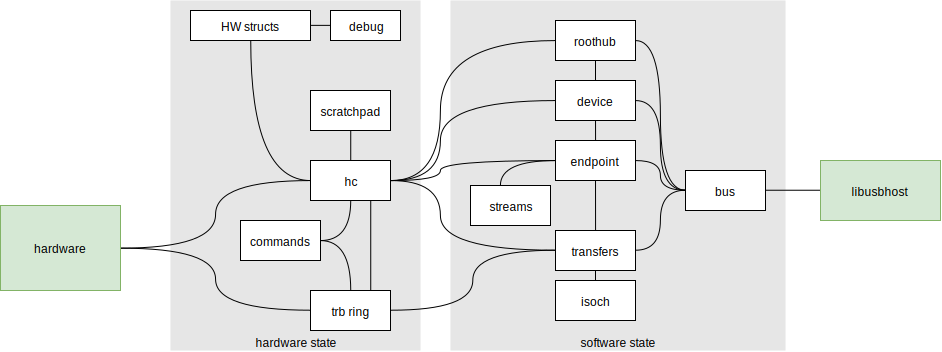
\includegraphics[width=0.8\textwidth]{xhci-architecture}
	\caption{The modules of xHCI driver}
\end{figure}

The scheme is not at all strict, we're in a C world, there are dependencies
almost everywhere -- take it as an informal overview to get an idea.

The whole driver can be split into two parts. The left one takes care about the
hardware perception on what's going on, the right one is about managing the
software structures and memory.

We start with describing the modules in the hardware part, as their
functionality is clear. Their order follows the order in which they were
implemented.

\section{HW structs}

% TODO: Explain that this one is really simple, and just mirrors the structures
% hardware use.

\section{Debug}

% TODO: Describe that we used it during debugging to check what we're doing.

\section{TRB ring}

% TODO @aearsis: explain the TRB rings, what they do and how they're
% implemented (ْ±2 pages, bore the reader to death right now!)
\subsection{Purpose}
\subsection{Implementation}

\section{Scratchpad}

% TODO: Anyone please explain these. The only interesting part is how the
% number of buffers are split weird and how we needed several attempts to get
% it right :)

\section{Events}

% TODO: Explain events, event handling and the event ring.

\section{Commands}
\label{sec:commands}

The xHC offers an independent command interface. During operation, the xHC
driver uses this interface to manipulate device slots, devices and endpoints by
executing various commands provided by a unified command subsystem. This
section provides details on the structure and implementation of this subsystem.


\subsection{Execution Workflow}

The xHC command interface consists of a TRB command ring and a command doorbell
register. Commands are executed by placing various command TRBs onto this ring,
forming a \textit{Command Descriptor}.

After placing the respective TRBs and writing to the xHC command doorbell
register, the descriptors on the command ring are sequentially processed by the
xHC, resulting in either failure or successful completion. The result of every
command descriptor is reported back to the xHCI driver in the form of a
\textit{Command Completion Event} placed onto the primary event TRB ring.

After writing into the xHC command doorbell register and before receiving the
respective command completion event, the xHCI driver can attempt to abort the
issued command. Such action might be of use for instance if the command
completion event does not arrive within a set time period.

Note that this section intentionally omits hardware technical details, which are
not instrumental in understanding the command subsystem. For further hardware
documentation of the xHC command interface, refer to \xhci{4.6}.


\subsection{Structure}

The xHCI driver command subsystem instance is represented by the
\struct{xhci_cmd_ring_t} structure which exists throughout the entire duration
of the xHCI driver's lifecycle. The purpose of this structure is to maintain and
manage the command TRB ring and to keep track of enqueued command descriptors.

Individual command descriptors are represented by the \struct{xhci_cmd_t}
structure. In this structure are stored high-level parameters of the command as well as
the command TRB, which is placed onto the command ring when the command is
executed. While the high-level command parameters are kept directly in this
structure, the hardware-related internals are kept in a substructure, which is
commonly referred to as \textit{command header}. The purpose of this separation
is to stress that the header contents are to be exclusively accessible to the
command subsystem, while the rest of the structure remains accessible to
the entire xHCI driver.

Besides data structures, the command subsystem offers a centralized command
completion event handler function -- \fnc{xhci_handle_command_completion} --
which is called by the event subsystem in case a \textit{Command Completion
Event} is encountered.

The last major component of the command subsystem are functions used to generate
and schedule commands on the xHC. These functions produce valid instances of the
\struct{xhci_cmd_t} and place their respective TRBs onto the command ring
managed by the \struct{xhci_cmd_ring_t} structure, requesting either blocking or
non-blocking semantics for waiting on their completion. These functions are
described in detail in the next section.


\subsection{Command Lifecycle}

\subsubsection{Issuing Commands}

By design, the internal logic of the command subsystem is kept opaque with
respect to other components of the driver. A notable example of this is the
mechanism for command scheduling.

Commands are usually issued by the HC component of the xHCI driver. At the time
of issuing, the information required can be broken down into three groups:
%
\begin{description}
	\item[Command Type]
		One of the 15 commands supported by the xHC command interface.
	\item[Command-specific Parameters]
		The number, type and semantics of these parameters depend on the
		specified command type.
	\item[Completion Semantics]
		This is the desired behavior of command execution.

		In the \textit{blocking mode}, the call to issue the command will block
		the calling fibril until the completion event is received.

		On the other hand, in the \textit{non-blocking mode}, the fibril will
		only be blocked until the command is issued -- the command subsystem
		will take the ownership of the command and deallocate it when the
		completion event arrives. This mode is meant for commands which do not
		require completion event handling and involves more complicated memory
		management since the command subsystem is responsible for freeing the
		command after the completion occurs.
\end{description}

Depending on the desired completion semantics of the issued command, the HC
component calls either the \fnc{xhci_cmd_sync} or \fnc{xhci_cmd_async}
function and passes it a configured instance of the \struct{xhci_cmd_t} structure.
Upon such call, the command subsystem will execute an internal command handler
function, which copies the high-level command-specific parameters configured by
the issuer, and use their values to construct a command descriptor consisting of
TRBs.

At this point, the \struct{xhci_cmd_ring_t} structure is modified and the new
command descriptor is placed onto the TRB ring. The corresponding instance of
\struct{xhci_cmd_t} is added to the active command list and depending on the
completion semantics, the issuing fibril is either suspended or continues
execution regardless of the completion event.


\subsubsection{Handling Completion}

When a command is completed, a \textit{Command Completion Event} is generated by
the xHC. This event is detected by the event subsystem, which in such case
triggers the \fnc{xhci_handle_command_completion} function.

This function extracts the address of the completed command descriptor and uses
it to find a matching instance of the \struct{xhci_cmd_t} structure in the
active command list.

Depending on the desired completion semantics, the command subsystem either
wakes the sleeping issuer fibril, or discards the non-blocking command from the
memory.


\subsubsection{Aborting Commands}

The command subsystem defined by xHCI contains a mechanism to trigger early
command abortion. It is not guaranteed to be effective for all commands, just
for commands control of which is out of HC's hands. A good example might be the
\macro{SET_ADDRESS} command, which issues the USB control request
\emph{SetAddress}, and waits for the device's response. Such command blocks
until the response is received. If the software, for any reason, wants the
command to be aborted, it can write 1 to the \macro{CA} bit of the
\emph{Command Ring Control Register}.

When the HC is triggered by a command abortion, it places a \emph{Command Ring
Stopped} event on the primary event ring and halts command processing. The ring
can be started again by ringing its doorbell. If a command was actually
aborted, a corresponding \emph{Command Completion Event} with status
\emph{Command Aborted} is placed first.

We decided to set a fixed timeout for every command, regardless of its
possibility to block, arbitrarily chosen as 10 seconds. That gives a generous
amount of time for the HC to finish a command. When this timeout is over,
a command is aborted.

Here comes the catch: the driver is not able to choose which command is to be
aborted -- it is always the one currently processed. Usually, it's the one that
blocks the pipe, but it means that the driver cannot simply place a timed
constraint on a command execution. To reflect the hardware semantics, all
fibrils that expire the timeout behave the same: they trigger a command
abortion, wait for the command ring to be stopped, then start it again.

To orchestrate several fibrils trying to schedule new commands, waiting for
commands to be completed and also the one handling an interrupt, a simple state
machine with synchronization is incorporated. In case the command ring is
being restarted, newly issued commands are delayed to prevent the doorbell from
being rung unexpectedly. When there are multiple fibrils with an expired timeout
while the abort is already triggered but not yet finished, they retract and
wait for the full timeout period again.

That common execution path is enclosed within a function called
\fnc{try_abort_current_command} (static for the command subsystem). As it's hard
to force a command to stall, we haven't had many opportunities to test the
behavior. Usually, the mechanism was triggered by a deadlock in our code, which
didn't magically disappear when a command was aborted. Also, the commands
always finish on time in a virtual environment. At the time of writing this
documentation, there has been only one observed legitimate occurrence of
a command stall on real hardware. The abort mechanism did its job well that day.

\subsection{Usage Examples}

Since the command subsystem is used at a multitude of places in the HC
component, it has been the goal of the authors to make its usage elegant and
effortless. For that reason, a dedicated inline notation syntax powered by
preprocessor macros has been devised and implemented. This is demonstrated in
Listing \ref{lst:command-usage}.

\begin{listing}[h]
	\begin{code}
		xhci_hc_t * const hc;

		/* Issue a "Set TR Dequeue Pointer" command synchronously. */
		const int result = xhci_cmd_sync_inline(hc, SET_TR_DEQUEUE_POINTER,
		    /* Command-specific arguments use struct initializer. */
		    .slot_id = slot_id,
		    .endpoint_id = dci,
		    .stream_id = stream_id,
		    .dequeue_ptr = addr,
		);

		/* At this point, the command is completed with `result`. */
	\end{code}
	\caption[Usage example of xHCI driver inline command syntax.]{Usage example
	of the xHCI driver command subsystem inline  syntax. This snippet issues a
	\textit{Set TR Dequeue Pointer} command to the HC in blocking mode. Note
	that the command initialization, configuration and finalization is handled
	by the inline macro syntax.}
	\label{lst:command-usage}
\end{listing}



\section{Host controller module}

% TODO: This will be harder, this one is a mix of what didn't fit anywhere else.
% Ideas:
% - event handling
% - context management
% - extcap parsing
% - register access macros

\section{Roothub}

% TODO: Explain why we do not have virthub. Who remembers the reasons?
% Otherwise it just uses libusb/port to do the interesting work.

\section{Transfers}

% TODO @salmelu (probably?): Write something about it.

\subsection{Isochronous transfers}

% TODO @salmelu: Copy that from the wiki :)

\section{Bus module}

% TODO: After the device will be split, will there be anything interesting to write about?

\subsection{Device}

% TODO: Enumeration, device context

\subsection{Endpoint}

% TODO: Contexts, rings

\subsection{Streams}

% TODO @salmelu: Noone else understands that now.

\chapter{USB Subsystem Modifications}
\label{usb-refactoring}

% TODO

\section{Explicit Device Removal}

One of the project goals is to alter the USB subsystem to allow support for
explicit device removal. Such feature can be found in most modern operating
systems and is often used to ensure that devices are left in a consistent state
after a physical port detachment occurs.

The explicit device removal feature usually provides a frontend interface in
the operating system, through which users can observe currently connected
devices and, if needed, issue a signal to the operating system that their
physical detachment is imminent. Following that, the system is expected to
promptly terminate all ongoing communications with the device and signal the
user back. After receiving the confirmation, user can then safely unplug the
device from the system bus without any risk of interrupting communications,
which could otherwise result in undefined state of the device.


\subsection{Considerations}

In the USB protocol, communications between the host and the device take place
in the form of \textit{transfers}. Depending on its version, the host controller
may have various roles in the realization of these transfers. For that reason,
version-specific modifications are carried out separately in host controller
drivers, whereas common functionality is implemented in the bus module, which is
a part of \lib{libusbhost}.

The disconnection routine for explicit device removal is implemented as follows:
~
\begin{enumerate}
	\item The user signals the intention to disconnect a USB device.
	\item The respective device drivers are notified to end their business (e.
		g. flush buffers or close files), possibly scheduling a multitude of
		transfers to the device.
	\item The HC driver disables the capability to schedule new transfers to the
		device.
	\item The HC driver aborts all leftover active transfers to the device.
	\item The device configuration is dropped, leaving it in the
		\state{Addressed} state, in which it is considered safe to be
		physically removed from the bus.
\end{enumerate}

If the user requests that this routine is rolled back, the steps of the
disconnection routine are just executed in reverse order. The following can
therefore be labeled as a reconnection routine:
~
\begin{enumerate}
	\item The user signals the intention to resume communications with a USB
	device, on which the disconnection routine has been previously performed.
	\item The HC driver configures the device.
	\item The HC driver enables the capability to schedule new transfers to the
	device.
	\item The operating system is notified that the device is reachable and
	matches it to appropriate drivers, which initiate communications with it.
\end{enumerate}

The specialization of both routines is performed in the same way as other bus
module interactions. All HC drivers hand off their DDF and device callbacks to
the bus module, which then calls them back to perform low-level commands related
to specific devices, endpoints and transfers. This way, the high-level logic
contained by the bus module essentially follows the listed descriptions above
and the version-specific extensions are resolved in the respective HC driver
implementations.


\subsection{Offline and Online DDF Signal}

The HelenOS Device Driver Framework includes two user-initiated signals
relevant to the implementation of this feature.

\begin{description}
	\item[Offline Signal]
		This signal informs a driver attached to a DDF node that its managed
		device may be removed in the near future. The driver is expected to
		immediately cease all user operations on the device and unbind its
		child DDF functions, possibly sending a \textit{Device Remove} signal
		to all their attached drivers in the process.

	\item[Online Signal]
		This signal is a logical counterpart to the previous signal.
		It informs a driver attached to a DDF node that its managed device will
		not be removed in the near future. The driver is expected to expose all
		child DDF functions related to the device, possibly sending a
		\textit{Device Add} signal to all their matched drivers in the process.
\end{description}

These signals can be easily issued by the user from the system shell by means
of the \app{devctl} application. See Listing \ref{lst:devctl-offline-online}
for invocation example.

\begin{listing}
	\begin{bdsh}
		# Prepare the unplug high speed device at address 2.
		devctl offline /hw/pci0/00:04.0/usb2-hs

		# We changed our mind. Bring the device back online.
		devctl online /hw/pci0/00:04.0/usb2-hs
	\end{bdsh}
	\caption[Example usage of \app{devctl} to issue offline and online
	signal.]{Example usage of the \app{devctl} application to issue offline and
	online signal to a USB high speed device at address 2. The host controller
	PCI address is \texttt{00:04.0}.}
	\label{lst:devctl-offline-online}
\end{listing}

It follows that these signals can be used for the implementation of the
explicit device removal at the level of USB host controller drivers. For that
reason, \lib{libusbhost} has been extended to handle appropriate DDF callbacks
for functions corresponding to HC's child devices. Their handling is forwarded
to the bus module, which executes the disconnection or the reconnection routine
for the \textit{offline} and \textit{online} signal respectively. In addition,
the transfer scheduling mechanism of the bus module has been extended to permit
scheduling new transfers only to devices, which are in the online state.

The general scheme of stopping communication with a device breaks down to
unregistering all its registered endpoints. The biggest challenge the driver
faces is to abort all currently running transfers on an endpoint that is being
unregistered. The majority of transfers (Bulk, Control, Isochronous,
Interrupt-out) wouldn't pose a problem -- we could just wait the short while
until they are completed, either successfully or not. But then there are
Interrupt-in transfers, which, especially in case of gone device, may not
complete in a timely manner.

\subsection{Aborting Active Transfers}

It is not possible to ``abort a transfer'' in a generic way, mainly because of
synchronization issues. Before we explain how can a transfer be properly
aborted in various Host Controllers, let us describe the lifecycle of
a transfer batch, a structure representing a transfer in HC drivers.

Currently, USB stack in HelenOS only supports synchronous interface to interact
with pipes. The two methods are called \fnc{dev_read} and \fnc{dev_write}.
Driver calls these methods on pipes, and provides a buffer -- either filled
with data, or to be filled. Once the call crosses the IPC barrier, it is joined
to a call to \fnc{bus_device_send_batch}. This function finds the target
endpoint structure, and passes control to \fnc{endpoint_send_batch}.

There, an instance of \struct{usb_transfer_batch_t} structure is created and
filled with parameters of the transfer. It is then passed to the driver
implementation to be scheduled. The driver typically copies the data to
a buffer suitable for the device, prepares some supporting structures, and
finally, schedules the transfer to the hardware.

Since then, an interrupt may come and finish the transfer in a different
fibril. A transfer is finished by copying the data out from the hardware buffer
to the batch buffer, setting the error code and calling a completion callback.
This callbacks answers the original incoming IPC call, causing the \fnc{dev_read/write}
function to return. After that, the transfer batch is destroyed.

But that's not the only scenario that may happen. From the moment a transfer is
created, a pointer to it must not be forgotten, otherwise the caller would
never return. But on the other side, once the pointer to batch is stored
somewhere, the transfer might be aborted at any time. Furthermore, once the
transfer is scheduled to the hardware, the buffers must not be deallocated
until the driver is sure that the hardware won't use them anymore.

This synchronization problem might be resolved by locking the batch and
reference counting, but then different problems would arise (e.g. a transfer
could be finished after the endpoint was successfully unregistered, just
because we cannot know if there's any). So, we decided to take a different
approach.

As the interface is synchronous (and it doesn't make much sense to make it
asynchronous, unless under special conditions), and the endpoint is assumed to
be available for one driver only, there's no point in having more than one
transfer active at a time. So, we store the pointer to a batch inside the
endpoint structure, in the field \struct{active_batch}. This field shall not be
accessed, unless the endpoint guard is locked.

Speaking about the endpoint guard leads us to one of the strange design
decisions we made. Endpoints do not have their own guard, they inherit one
while being put into the online state. That is, when the endpoint is being
registered, the HC driver calls \fnc{endpoint_set_online} and passes a pointer
to a mutex which will be used to synchronize transfers on that endpoint. The
endpoint itself never locks this mutex, it only uses it to ensure correctness
(whether the mutex is locked in named functions) and to wait on a condition
variable.

Sooner or later in the scheduling of a transfer batch, there is a need to access
shared structures. Once there is, the HC driver locks the mutex, and in a single
critical section it calls the function \fnc{endpoint_activate_locked}. If this
function successfully returns, the endpoint is reserved for a given batch. By
calling the function, the batch ownership is given to the endpoint -- once the
critical section ends, the batch must be considered already finished.

In the meantime, there are two possible execution flows that are related. First
of all, there is the interrupt handler finishing transfers. Once it decides
a transfer is to be finished, it is supposed to have the mutex already locked
(to avoid racing with the scheduling fibril), and calls function
\fnc{endpoint_deactivate_locked}. This function allows another batch to use the
endpoint, and transfers the ownership of the batch to the caller.

Second, there can be a fibril trying to unregister the endpoint. To do so, it
locks the mutex, and calls \fnc{endpoint_set_offline}. This blocks access for
further transfers, and also wakes fibrils waiting inside
\fnc{endpoint_activate_locked} from the sleep, returning an error value. The
unregistering fibril then may decide to wait a while to finish already running
transfers, and then do HC-specific steps to remove the running transfer from the
hardware. Eventually, it shall call \fnc{endpoint_deactivate_locked}, which
takes the ownership of the batch, and gives the unregistering fibril a sole
right to finish the transfer with an error code.

This whole mechanism is completely opt-in, and the driver can avoid using it
(like xHCI do for stream-enabled endpoints). The HC-specific part of the
implementation is discussed in the next sections.

\subsection{UHCI, OHCI and EHCI Specifics}

All three HCI's that were supported prior to our project have similar
structure with regard to what is required to implement transfer aborting. Let us
first describe very briefly how these controllers handle transfers.

Generally, all three host controllers require the driver to create a system of
linked structures in memory (for UHCI and OHCI, restricted to the lower 4 GBs
of addressable space). The names and guts differ, the structures however
describe a linked chain of queues. Queues are then filled by transfer
descriptors, which describe USB transfers to be done. Once the transfer is
done, its descriptor is flagged, removed from the queue and if the descriptor
is marked, the host is interrupted. More specific information can be found
either in respective specifications, or in the documentation of the HelUSB
project.

At the time of receiving an interrupt, the host does not know which transfer
was finished, so it has to check all pending transfer descriptors for the
completion flag. In case all the transfer descriptors of a transfer are
completed, the driver may finish the transfer.

When aborting a transfer, the driver must make sure the controller is not using
any of the allocated buffers. It is allowed to modify the queues while the
controller is scanning them, the modifications must however follow an order in
which the consistency of the structure is guaranteed at any time. After it
does, it must notify the driver that the structure has changed, in order to
force the controller to clear its caches (EHCI only).

Because the interrupt handler is polling the transfers for completion, it is
enough for the driver to remove the transfer from the list of pending transfers
to be sure no other fibril will ever complete it. After that, we can finish it
ourselves with an error. Note that in this case it is unknown to driver whether
the transfer was completed or not -- but since the driver is unregistering an
endpoint, the device must already be in a state in which it expects removal.

The nature of handling finished transfers defines the weird semantics of the
inherited mutex. Let's consider a situation, in which two locks were involved:
a lock protecting the HC structures (lists, interrupt handling, \dots) called
$H$ and a lock protecting the endpoint $E$. When a transfer is scheduled, it
must first wait until the endpoint is available. To avoid a deadlock between
finishing the current transfer and waiting for it to finish, the mutex $E$ must
be taken first. Also, $E$ cannot be released before taking $H$, because after
$E$ is released the transfer can be aborted immediately. On the other hand, when
an interrupt comes, there is no way how to get a pointer to the endpoint without
taking $H$ first. Neither $H$ cannot be released before taking $E$, because
we cannot access the batch unless holding $E$, and even transferring a pointer
to an endpoint does not help -- in between the critical sections the current
transfer transfer can be aborted and a new one scheduled, resulting in
completing a wrong transfer. To avoid ABBA deadlock eventually, we just have to
avoid using two locks for transfer synchronization.

From the further perspective, these controllers do not have an internal state
for individual devices and endpoints, so the deconfiguration and its rollback
is an operation on software-state only. As such it is already done completely
by the \lib{libusbhost} library.

\subsection{xHCI Specifics}

Since xHCI is the latest HC interface implementation, a lot more is done by the
hardware for the HC driver in comparison with previous versions. The concept of
xHCI command ring leads to very elegant implementation of the required
functionality on the HC driver part.

For the purpose of aborting active transfers, the xHCI features an explicit
\textit{Stop Endpoint} command, which instructs the HC to abort all transfers
to a specific device endpoint. This command is issued by the HC driver for all
removed device endpoints, which are active at the moment of the request.
Furthermore, device configuration is dropped along with all remaining endpoints
by issuing a \textit{Configure Endpoint} command with the DC (deconfigure)
flag.

Reconnection is quite straightforward and requires only that the HC driver
issues a regular \textit{Configure Endpoint} command in order to transition the
device from the \state{Addressed} state back to the \state{Configured} state.


\subsection{Driver Support}

Since the existing USB drivers were quite incomplete, their implementation has
been extended to add support for explicit device removal. This mostly lead to
novel approaches to deallocation of device-related memory structures, which is
often performed in the \fnc{device_remove} and \fnc{device_gone} driver
callbacks.

For instance, a number of drivers required that an implementation of
\fnc{device_remove} is created in the first place. Quite so often, the
existing implementation of \fnc{device_gone} has provided a good starting
point, given that both functions have to deal with USB device's demise. The
fundamental difference was that while \fnc{device_gone} merely dealt with
the fallout of unexpectedly unplugged device, \fnc{device_remove} had the
opportunity to tie up all lose ends prior to the physical detachment of the
device.

This posed a problem, especially in HID and hub drivers, which heavily relied on
polling of interrupt endpoints. Since polling was a synchronous operation from
the device driver's point of view, a polling fibril has been created when the
driver started managing the device. When the device was unplugged, the polling
operation failed with an error, waking up and effectively terminating the fibril in
the process. Since no explicit joining mechanism was available, the
implementation of \fnc{device_gone} merely spinned a limited number of times,
waiting for the polling fibril to die. This mechanism was however unsuitable for
\fnc{device_remove}, since the fibril would not awaken due to an error caused
by the physical disconnect, which has not happened yet.

This lead to complete refactoring and extension of the USB device polling
mechanism, which is described in detail in Section \ref{polling-refactoring}.
In summation, the new version of the mechanism allows device drivers to join
their polling fibrils and consistently wake them up in order to avoid deadlocks.

To actually stop the polling in the \fnc{device_remove} callback, the device
driver has to trigger a transfer abort inside the HC. There's no sensible way
of how to allow a driver abort its own transfer, which wouldn't introduce
potential memory leaks inside HC or synchronization problems. So we decided
that the driver will have to unregister the endpoint as the only way to abort
a currently running transfer (and also disable scheduling of new ones). The
device's endpoints (or, at this layer already called pipes) are completely
managed by the \lib{libusbdev} library. Previously, their lifetime was strictly
tied to the lifetime of the handled device. There are only two possible
ordering of these two operations:

\begin{enumerate}
	\item Close the pipes after the \fnc{device_remove} callback returns.
		After that, the polling fibrils will end and destroy their structures.
		The library USB device structure will have to be reference-counted and
		the counter will be managed by the driver to account for polling
		fibrils.

	\item Close the pipes prior to calling \fnc{device_remove}, effectively
		destroying the only reason why this callback exists, and make the
		expected removal equivalent to the unexpected one.
\end{enumerate}

\noindent It is pretty obvious that we had to choose a completely different approach. So
we came up with three more options:

\begin{enumerate}
\setcounter{enumi}{2}
	\item Introduce a new callback, e.g. \fnc{device_removed}, to be called
		after the pipes are closed. The removal would be split into two phases:
		first, in \fnc{device_remove} the loose ends are closed and the
		device is brought to a state expecting removal, then in
		\fnc{device_removed}, the polling fibrils are joined and structures
		are destroyed.

	\item After calling \fnc{device_remove} and closing the pipes, call
		\fnc{device_gone}.

	\item Allow the driver to close individual pipes imperatively.
\end{enumerate}

At first, we decided to go with option 3). But it was yet another callback, we
didn't come up with a name that wasn't so similar and yet was clear, and
finally, the \fnc{device_removed} callback implementations were very similar
to \fnc{device_gone}.

The option 4) seems reasonable at the first look, but it would create
inconsistency between DDF drivers and USB drivers, which would be very
confusing for developers. \footnote{Actually, some team members think this
behavior shall be present in DDF too, but we didn't open a discussion with
HelenOS developers.}

In the end, the only option left was letting the driver close its own pipes. So
we introduced a new library call \fnc{usb_device_unmap_ep}, which does
exactly that. The new library polling mechanism closes its pipe automatically,
but this functionality is usable in any driver for any endpoint.

The implementation of explicit device removal support for the rest of the
drivers was a trivial extension of their previous functionality.


\section{Polling Mechanism Improvements}~\label{polling-refactoring}

As hinted by the previous section, the USB device endpoint polling mechanism has
been completely refactored.


\subsection{Before State}

In the original state, USB device drivers had to configure polling using a
configuration structure \struct{usb_device_auto_polling_t}, then pass this
structure to one of four functions:

\begin{itemize}
	\item \fnc{usb_device_auto_poll()},
	\item \fnc{usb_device_auto_poll_desc()},
	\item \fnc{usb_device_auto_polling()},
	\item \fnc{usb_device_auto_polling_desc()}.
\end{itemize}

These functions copied the configuration and started an automated polling
fibril, which interacted with the deice driver using callbacks specified in the
configuration structure. At the end of the polling, the fibril deallocated all
of the resources and terminated.


\subsection{Motivation}

There was a number of problems with the status quo:

\begin{itemize}
	\item The semantics of functions used to initiate polling was not clearly
		distinguished by their name (and neither their documentation).
	\item In addition, the polling functions had a high number of arguments,
		which opened possible room to device driver errors due to their
		misinterpretation (or further API changes in the future).
	\item The polling fibril was detached at the moment of polling start and
		could outlive the device in the driver's memory, then fail later when
		accessing memory, which was already freed in \fnc{device_remove()} or
		\fnc{device_gone()}. Some drivers bypassed this by spinning in these callbacks,
		waiting for the fibril to terminate. However, if the fibril was still
		polling even after a number of attempts, a non-zero error code was returned,
		rendering the entire DDF function (along with its subtree) in a defunct
		state.
	\item The driver was unable to inspect the state of the polling fibril
		directly, so often a flag had to be created and maintained by polling
		callbacks.
	\item A distinct subset of polling parameters were not configurable and were
		hard-assigned their default values inside function implementation. If the
		driver wanted to change any (and not necessarily all) of such parameters, it
		had to specify all the values by itself. Because the constants were
		hard-coded in the implementation, the driver then usually had to copy the
		values.
\end{itemize}


\subsection{Modifications}

\begin{figure}
	\centering
	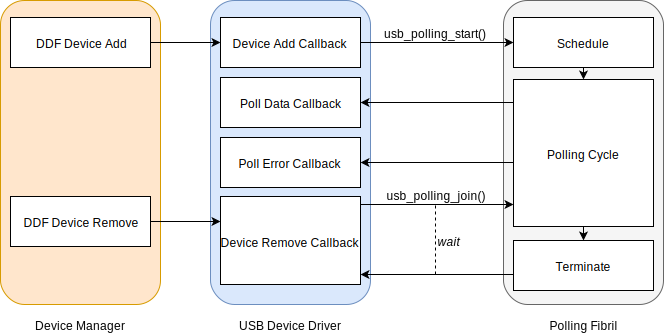
\includegraphics[width=0.8\textwidth]{usb-polling}
	\caption[USB device polling interactions diagram.]{A diagram of interactions
	between the Device Manager, USB device driver and one of its polling fibrils
	during its lifecycle.}
	\label{fig:usb-polling}
\end{figure}

The configuration structure \struct{usb_device_auto_polling_t} has been renamed
for simplicity sake to \struct{usb_polling_t}. Instead of serving as a one-time
configuration structure during polling initiation, its role changed to represent
the entire instance of the polling process throughout its lifetime.

Introducing standard functions such as \fnc{usb_polling_init()} and
\fnc{usb_polling_fini()}, the device driver is now fully responsible for the
ownership of the structure. This is convenient, since drivers often have their
own structures for device data, where \struct{usb_polling_t} can be placed as a
field, dropping the need for additional calls to \fnc{malloc()} and
\fnc{free()}. In addition, this resolves the problem with default values of
various configuration parameters, since in \fnc{usb_polling_init()} all
parameters are assigned their default values and device driver can override only
those desired.

All four of the original polling initialization functions were unified into a
single function \fnc{usb_polling_start()}. Since there is now a clear structure,
which represents the polling instance, the arguments of the original four
functions were moved to \struct{usb_polling_t}, where they are clearly named and
documented, preventing any possible errors from their misinterpretation. Suffice
it to say, that the original four functions mostly fulfilled the role of syntax
sugar, which is now rendered unnecessary, given the fact that default values of
configuration parameters are pre-filled in the polling structure.

Lastly, the API was extended with the \fnc{usb_polling_join()} function, which
closes the polling pipe and consistently waits until the polling fibril
terminates. This function addresses the problem of spinning in driver's
\fnc{device_remove()} or \fnc{device_gone()} callbacks, or possible negligence,
which may result in the polling fibril outliving the device and then accessing
invalid memory. Calling this function in this context will result in the
immediate and synchronous termination of the polling mechanism prior to
deallocation (as depicted in Figure \ref{fig:usb-polling}).

Furthermore, the exposure of internal polling parameters now gives device
drivers more creativity in their approach to polling. For instance, drivers can
now inquire about the state of the polling fibril without the need to have a
private flag maintained by their polling callbacks. The drivers can also change
polling parameters such as request size or polling delay mid-flight, which is a
more flexible approach than to stop polling, change parameters and then start
polling again (note that stopping polling at will was not supported by the
previous implementation without generating actual errors from the hardware
device).

A nice minimalist example of the new polling mechanism usage can be found in
Listing \ref{lst:polling-example}

\begin{listing}
	\begin{code}
		static usb_polling_t polling;
		static uint8_t buffer[13];

		static bool callback(usb_device_t *dev, uint8_t *buffer, size_t size, void *arg)
		{
			printf("Have data!/n");

			// Return true if we wish to continue polling.
			return true;
		}

		static void demo()
		{
			// Initialize.
			usb_polling_init(&polling);

			// Configure.
			polling.device = /* some usb_device_t here */;
			polling.ep_mapping = /* some interrupt(in) endpoint of the device */;
			polling.buffer = buffer;
			polling.request_size = sizeof(buffer);
			polling.on_data = callback;

			// Start polling.
			usb_polling_start(&polling);

			// Sleep synchronously for a while.
			async_usleep(10000);

			// End polling and clean up.
			usb_polling_join(&polling);
			usb_polling_fini(&polling);
		}
	\end{code}
	\caption{Minimal usage example of the new USB device polling mechanism.}
	\label{lst:polling-example}
\end{listing}




\chapter{Writing USB Drivers}

This chapter provides documentation and general guidelines for usage of the
refactored USB device driver interface. As such, it is meant for developers of
HelenOS device drivers, who can use it as a reference guide. By intention, this
section abstracts the reader from all modifications to the stack, and focuses
only on the latest state of the interface. All changes to the interface are
described in detail in Chapter \ref{usb-refactoring}.

The reader should note that there exists a similar section in the initial USB
stack documentation. The text in this chapter could be considered an updated
version or extension of that text.


\section{Basics}
This section gives details on the basic structure of USB device drivers, their
role in the system and components they usually interact with.


\subsection{Framework}
USB device drivers use the generic \textit{Device Driver Framework} available in
HelenOS. Because all USB drivers have similar initialization routines, a thin
layer -- specific to USB devices -- was added above the generic one. This layer
mainly serves as a middleware for easy communication with USB host controller
drivers, performing USB specific resource management and enabling device drivers
to initialize endpoint pipes and interact with USB devices. For those reasons,
USB device drivers are recommended to link with \lib{libdrv} and
\lib{libusbdev}, which contain both aforementioned layers respectively.

It is expected that USB device drivers specify in advance not only their
relevant match identifiers, which are used by the Device Manager to pair new
devices with available drivers, but also all endpoints, which shall be present
on the device through a USB driver structure. Later when a new device is found,
a specialized device structure is prepared and pipe abstractions are
initialized.

Device drivers live the same life cycle as any other drivers controlled by the
\textit{Device Manager}. A quick summary follows:
~
\begin{enumerate}
	\item The driver is started at the convenience of the Device Manager if and
	when a compatible device is found. At startup, the driver registers with the
	USB framework, which in turn registers also with the Device Driver
	Framework.

	\item During its lifetime, the driver receives IPC callbacks from the USB
	Framework, informing it about relevant device events. On the basis of these
	events, the driver then communicates with the device and exposes various
	interfaces to other tasks in the system. At this point, the controlled
	device usually becomes visible and useful to the user.

	\item When there is no more need for the driver to run (i.e. no devices to
	control), the Device Manager terminates the driver to save resources.
\end{enumerate}

In the Device Driver Framework, drivers are the consumers of \textit{devices}
and providers of \textit{functions}. This paradigm allows them to expose an
unlimited number of nodes (representing logical or physical units) for every
device they control. The same basic principle holds for USB drivers as well.


\subsection{Device Callbacks}
As explained in the previous section, USB device drivers are informed about
relevant device events by asynchronous IPC callbacks from the USB framework. To
simplify usage, these callbacks are identical to those of the Device Driver
Framework:
~
\begin{description}
	\item[Add Device] This event notifies the driver that a new device has been
	discovered and matched to it. From this point on, the driver is allowed to
	communicate with the device in order to configure it and expose its
	functions to the rest of the system. Further communication with the device
	will likely depend on remote calls originating from other system tasks
	utilizing the exposed interface.

	\item[Remove Device] This event instructs the driver to immediately disallow
	new user operations on a device, terminate all currently running
	operations in a timely manner, and hand device control back to the system,
	as the device will likely be physically removed from the bus in the
	forseeable future.

	\item[Device Gone] This event informs the driver that a device has been
	physically disconnected from the system without a prior \textit{Remove
	Device} event. Since the device is no longer reachable, the driver is to
	force interrupt all user operations, which were running at the time of
	receiving the event and report failure to the callers.
	
	\item[Offline Function] By receiving this event, the driver is asked by the
	system to explicitly transition a specific function exposed by one of its
	controlled devices into the \textit{Offline} state. The meaning of such
	transition might depend on the interpretation of the function. For more
	information, see the Device Driver Framework Documentation.

	\item[Online Function] By receiving this event, the driver is asked by the
	system to explicitly transition a specific function exposed by one of its
	controlled devices into the \textit{Online} state. Again, the meaning of such
	transition might depend on the interpretation of the function. For more
	information, see the Device Driver Framework Documentation.
\end{description}



\section{Device Communication}
% TODO

\subsection{Endpoint Mapping}
% TODO

\subsection{Pipes}
% TODO

\subsection{Automatic Polling}
% TODO


\section{Utilities}
% TODO

\subsection{Logging}
% TODO

\subsection{Descriptors}
% TODO

\subsection{DMA Buffers}
% TODO





% Appendices
\appendix
\chapter{Benchmarks and Testing}

To demonstrate and benchmark performance of the xHCI stack, a proprietary
subsystem has been implemented in HelenOS. The primary function of this
subsystem is to communicate with a custom QEMU USB device over arbitrary
endpoints and provide statistical information related to the communication.
This way, it can be used to verify the correctness of message transmission,
experiment with synchronization and to measure performance indicators.

In addition, since the subsystem is built on top of the USB device driver
framework and has no xHCI-specific requirements, it can be also used to compare
parameters of the xHCI stack with its predecessors.

The subsystem is composed of three parts:
~
\begin{description}
	\item[QEMU fork with proprietary diagnostic device (usb-tmon)]
		This implementation of QEMU contains a virtual USB device, which carries
		the diagnostic device class descriptor.
	\item[USB Diagnostic Device Driver (usbdiag)]
		The usbdiag driver matches with the QEMU diagnostic device and
		facilitates all communication with it. It also exposes a remote
		interface for all HelenOS applications.
	\item[User Frontend Program (tmon)]
		The tmon program is the primary user frontend in shell. It can use the
		interface exposed by usbdiag to perform various tests with diagnostic
		devices and return human-readable results.
\end{description}

\section{QEMU Device}

The \texttt{usb-tmon} virtual device is a diagnostic class USB device
created to allow us to test all of the different transfer types on one device,
gather data about the throughput and speed of the communication and validate
the contents of the USB packets sent between HelenOS and a device.

In order to support communications of all types, the device contains an
endpoint for each direction of each transfer type - i.e. interrupt, bulk and
isochronous. Since we want to both check the speed of the driver and the
correctness of the data sent, each endpoint is duplicated creating two
sets of endpoints - first set, which does not validate the transferred data,
and a second set, which checks that each four bytes of the data equal to a
predefined macro \macro{CHECK}. Each of these endpoints has an associated
macro that contains its endpoint number which has the form of
\macro{EP_<type>_<direction>} for the first set and
\macro{CHECKED_EP_<type>_<direction>} for the second set, where \texttt{<type>}
can be \texttt{INT} for interrupt transfers, \texttt{BULK} for bulk transfers or
\texttt{ISOC} for isochronous transfers and \texttt{<direction>} can be either
\texttt{IN} or \texttt{OUT}. Note that the way \texttt{usb-tmon} handles
transfers depends on the number of the endpoint, so the endpoint number used
by a driver has to match the value of one of these macros.

\subsection{Monitoring}

Regardless of which of the aforementioned endpoint sets is used, the
\texttt{usb-tmon} device prints information about the transfers it handles
to QEMU's standard output:
~
\begin{description}
	\item[Interrupt]
		Time since last \texttt{IN} or \texttt{OUT} interrupt request in
		microseconds.
	\item[Bulk]
		Amount of bytes transferred in the last second for every second of an
		\texttt{IN} or \texttt{OUT} bulk transfer.
	\item[Isochronous]
		Notification about receiving the request.
\end{description}

\subsection{Implementation}

The implementation of this device is located in the file
\qemufile{hw/usb/dev-tmon.c}{dev-tmon.c} in the helenos-xhci-team/qemu fork of
the official QEMU repository. It contains several key structures and functions:

\begin{description}
	\item[USBTmonState]
		Structure that represents the current state of a \texttt{usb-tmon}
		device.
	\item[desc\_tmon, desc\_device\_tmon, desc\_iface\_tmon]
		These three structures form the descriptor of the device and contain
		information about the device's class, protocol, endpoints etc.
	\item[usb\_tmon\_class\_init]
		Called when QEMU starts, so it is used as a constructor function for the
		virtual device and all relevant data.
	\item[usb\_tmon\_realize]
		Called when an instance of the \texttt{usb-tmon} device gets created and
		is used to initialize a specific instance of \struct{USBTmonState}.
	\item[usb\_tmon\_handle\_attach]
		Called when an instance of the \texttt{usb-tmon} device gets attached to
		the guest OS.
	\item[usb\_tmon\_handle\_control]
		Called when the device receives a control request, in its current
		implementation simply forwards the request to QEMU via
		\fnc{usb_desc_handle_control}.
	\item[usb\_tmon\_handle\_data]
		Called when the device receives an interrupt, a bulk or an isochronous
		data request, determines the receiving endpoint, stores information
		about handled data and if needed, sends or validates a USB packet.
	\item[usb\_tmon\_\{int\textbar bulk\textbar isoc\}\_\{in\textbar out\}]
		Called on specific kinds of transfers and track sent/received data.
\end{description}

These are the structures and functions one needs to modify in order to modify
the behavior of the device. Additionally, the source code contains helper
functions (e.g. time measurement with \fnc{get_now_sec} and \fnc{get_now_usec})
and QEMU debugging/informational functions and structures (e.g.
\struct{desc_strings}, \struct{vmstate_usb_tmon}, \struct{usb_tmon_info} and
\fnc{usb_tmon_register_types}). These should seldom require modification.

For the purposes of modifying or debugging usb-tmon's source code, the header
\qemufile{include/hw/usb.h}{usb.h} contains most of the structure definitions
and function declarations that might be needed.

\subsection{Usage}

To attach an instance of the \texttt{usb-tmon} device to a running QEMU, one
can type \textit{"device\_add usb-tmon"} into QEMU's monitor (which can be
accessed via the Ctrl-Alt-2 key combination or by redirecting the
monitor to QEMU's standard IO by adding \textit{"-monitor stdio"} to QEMU's
startup command). To have QEMU start with \texttt{usb-tmon} attached, they may
add \texttt{"-device usb-tmon"} to their QEMU startup command.

\section{Driver}

% TODO

\section{Frontend}

\subsection{Structure}

The \texttt{tmon} application consists of the following source files:
~
\begin{description}
	\item[\file{uspace/app/tmon/main.c}{main.c}]
		Main entry point, command selection and usage string.
	\item[\file{uspace/app/tmon/commands.h}{commands.h}]
		Executable commands.
	\item[\file{uspace/app/tmon/list.c}{list.c}]
		Implementation of the \textit{"list"} command.
	\item[\file{uspace/app/tmon/tf.h}{tf.h}, \file{uspace/app/tmon/tf.c}{tf.c}]
		Testing framework, common code for all "\fnc{test-*}" commands.
	\item[\file{uspace/app/tmon/resolve.h}{resolve.h},
		  \file{uspace/app/tmon/resolve.c}{resolve.c}]
		Resolving DDF device from string using devman's IPC interface.
	\item[\file{uspace/app/tmon/burst\_tests.c}{burst\_tests.c}]
		Implementation of burst tests.
\end{description}

\subsection{Usage}

\begin{bdsh}
tmon: benchmark USB diagnostic device

Usage: tmon command [device] [options]

      list - Print a list of connected diagnostic devices.
      test-intr-in - Read from interrupt endpoint as fast as possible.
      test-intr-out - Write to interrupt endpoint as fast as possible.
      test-bulk-in - Read from bulk endpoint as fast as possible.
      test-bulk-out - Write to bulk endpoint as fast as possible.
      test-isoch-in - Read from isochronous endpoint as fast as possible.
      test-isoch-out - Write to isochronous endpoint as fast as possible.

      -n --cycles
            Set the number of read/write cycles.
      -s --size
            Set the data size transferred in a single cycle.

If no device is specified, the first device is used provided that it is the
only one connected. Otherwise, the command fails.

\end{bdsh}

\chapter{Notes on Compatibility}

% TODO


\chapter{Future Development}

This chapter outlines features, which were considered optional extensions of
the project but were not realized due to time, complexity or other constraints.
These features provide good starting points for the future development of the
USB stack.

\section{Power Management}

The xHCI Specification focuses a lot on power management. Devices have multiple
states corresponding to the amount of power used, and links between devices
do so as well. Of course, to fully utilize these features, there must have been
a system-wide mechanism to declare intentions about power management. We are not
there yet.

Despite that, there are a few power switches we could toggle just now. Given the
small number of drivers implemented, we could for example make the USB fallback
driver suspend the device.

We consider power management a topic that needs to be addressed on the
system level, and as such we did not pay much attention to it.

\section{Asynchronous I/O}

The aspect we care about though is performance. Although the primary goal of
this project was to allow users to use USB on machines equipped only with xHC,
the performance benefit of USB 3 is not negligible, and could be well worth it.

Every transfer type of USB focuses on different characteristics of the
transfer. Interrupt pipes strive for the lowest latency possible -- in this
field, the synchronous semantics works very well. The latency between receiving
interrupts and delivering them as fast as an IPC reply to a call.

Considering isochronous endpoints, it is simply not possible to satisfy them
with a synchronous API. For that reason, we decided to change the semantics to asynchronous
one. The downside of the current approach is that the HC driver is forced to
copy the data out from the shared buffer, because its ownership is temporary.
But since isochronous transfers in xHCI are just a proof-of-concept and
there are no drivers for real devices yet, we have decided not to optimize
prematurely.

The bulk transfer type can however be utilized both synchronously and
asynchronously, and both use cases have their advantages as well as disadvantages. While synchronous API is easier to
work with, asynchronous would offer much better performance though. However, as there is just
a single driver using bulk endpoints, we have decided not to complicate matters and stay
with synchronous-only API for bulk pipes.

\section{Isochronous Transfers in UHCI+OHCI+EHCI}

The isochronous module implemented in xHCI can be thought of as a generic scheduling
framework for isochronous transfers. The scheduler behaves like a leaky bucket,
scheduling the transfers to xHC at a constant rate while throttling the device
driver. This is the most complicated part of handling isochronous transfers,
and implementing an asynchronous API for drivers is a good opportunity to
generify it for other drivers as well.

Implementing the support for isochronous transfers for older HCs is a bit
harder task, though. Those drivers use proprietary data structures for isochronous
transfers, and require the software to schedule transfers so all time
constraints are satisfied. (The xHC does it in hardware, and software is just
responsible for issuing transfers fast enough.) Also, because of a heavily
simplified implementation of periodic scheduling in the former HC drivers,
substantial refactoring is inevitable. That however requires a deeper
understanding of inner workings of individual HCIs.

\chapter{Project Specification and Timeline}

This section contains the original project specification, as it was approved by
the project committee at Faculty of Mathematics and Physics, Charles University.
The actual project realization timeline is also included.


\section{Project Specification (in Czech)}

\subsection{Základní informace}

\begin{description}
	\item[Jméno projektu] HelenOS USB 3.x Stack
	\item[Zkratka] HelUSB3
	\item[Vedoucí] Martin Děcký \email{decky@d3s.mff.cuni.cz}
	\item[Konzultanti] --
	\item[Anotace]
		Rozšíření podpory sběrnice USB a USB zařízení v mikrojádrovém multiserverovém operačním systému HelenOS o revizi 3.0 (resp. 3.1), sjednocení této podpory s dříve implementovanou funkcionalitou pro USB 1.0, 1.1 a 2.0 a další vylepšení.
\end{description}

\subsection{Motivace}

Podpora sběrnice USB v revizi 1.0 a 1.1, která byla naimplementována v rámci Softwarového
projektu v roce 2011 (HelUSB), výrazně rozšířila praktickou použitelnost operačního systému
HelenOS v souvislosti s periferními zařízeními. Na tuto funkcionalitu bylo později navázáno
podporou USB 2.0. V současné době je poslední specifikovaná revize USB 3.0 (z hlediska
hardwarového transportu potom 3.1) a začínají se objevovat počítače, které implementují pouze tuto
revizi (tedy z pohledu operačního systému nejsou zpětně kompatibilní se staršími revizemi). Proto
je vhodné, aby byl operační systém HelenOS doplněn o nativní podporu pro USB 3.0 (resp. 3.1).
Tento projekt je pochopitelně také vhodnou příležitostí pro provedení sjednocení s předchozími
implementacemi a provedení dalších souvisejících vylepšení.

\subsection{Popis projektu}

Primárním předmětem projektu je rozšířit generický framework pro použití USB sběrnic a
implementaci ovladačů USB zařízení v systému HelenOS o podporu USB revize 3.0 (resp. 3.1), při
zachování plné podpory předchozích revizí 1.0, 1.1 a 2.0. Cílem je, aby bylo možné na běžně
dostupném hardwaru využít nejvyšší možnou revizi USB s přihlédnutím k možnostem daných
periferních zařízení. Součástí projektu je také implementace základního demonstrátoru – ovladače
konkrétního fyzického USB host controlleru a ověření funkcionality konkrétních koncových USB
zařízení.

\begin{itemize}
	\item
		Implementace ovladače pro USB host controller podle normy xHCI.
		\begin{itemize}
			\item Podpora přenosových režimů a rychlostí odpovídajících USB 1.0, 1.1, 2.0 a 3.0.
			\item
				Enumerace zařízení na sběrnici USB 3.0 a spouštění příslušných ovladačů koncových USB zařízení (s využitím existujícího Device Driver Frameworku), jsou-li k dispozici.
				\begin{itemize}
					\item Zachování kompatibility s dříve naimplementovanými ovladači host controllerů podle norem OHCI, UHCI a EHCI.
					\item Ideálně zachování možnosti implementovat ovladače koncových USB zařízení nezávisle na použité variantě host controlleru.
				\end{itemize}
			\item Demonstrátor: Ovladač pro xHCI host controller NEC Renesas uPD720200
		\end{itemize}

	\item
		Implementace explicitního mechanismu odpojování USB zařízení (očekávaného i neočekávaného).
		\begin{itemize}
			\item Podpora přerušení USB komunikace (USB communication abort) na hardwarové úrovni bez zablokování ovladače USB zařízení.
		\end{itemize}

	\item Implementace podpory isochronního režimu komunikace USB zařízení.
	\item Volitelná část zadání: Rozšíření USB frameworku o dosud nepodporované vlastnosti (např. správa napájení), o podporu specifických xHCI host controllerů (např. Intel Sunrise Point-H a/nebo contollery integrované na vývojových deskách či SoC čipech typu BeagleBoard, BeagleBone, Raspberry Pi) či jiná vylepšení (např. implementace nových ovladačů koncových USB zařízení jako je DisplayLink, dokončení implementace správy přenosového pásma a výkonu, odladění ovladačů controllerů na jiných platformách).

\end{itemize}

\subsection{Platforma, technologie}

\begin{itemize}
	\item
	Framework a ovladače budou odladěny v simulátoru QEMU a na běžném fyzickém PC
	(obojí pro platformy x86 a x86-64) vybaveném výše uvedeným USB controllerem a
	případně kombinací již dříve podporovaných USB controllerů s použitím již existujících
	ovladačů koncových USB zařízení.

	\item
	Framework a ovladače budou implementovány takovým způsobem, který nebude
	principielně bránit jejich budoucímu využití na jiných platformách než x86 a x86-64.

	\item
	Framework a ovladače budou implementovány takovým způsobem, aby zachovávaly
	celkovou softwarovou architekturu mikrojádrového multiserverového operačního systemu
	HelenOS a aby nedošlo k omezení již dříve naimplementované a odladěné funkcionality (tj.
	podpora OHCI, UHCI atd.).
\end{itemize}


\subsection{Odhad náročnosti}

Na základě zkušeností z dřívějšího Softwarového projektu HelUSB (implementace podpory OHCI,
UHCI) lze říci, že zadání je řešitelským týmem o 5 – 6 studentech zvládnutelné ve standardní době.
Projekt klade na řešitele především následující nároky, ze kterých přirozeně plyne přibližný
harmonogram prací:

\begin{itemize}
	\item Nastudování specifikace sběrnice USB, specifikace xHCI, specifikace controlleru NEC Renesas uPD720200, volitelně studium implementací v jiných operačních systémech. [1 měsíc]

	\item Nastudování softwarové architektury, relevantních mechanismů a existující implementace systému HelenOS (async framework, Device Driver Framework, podpora OHCI, UHCI, EHCI). [1 měsíc]

	\item Implementace podpory xHCI a controlleru NEC Renesas uPD720200, integrace s existující implementací, refactoring. [2 měsíce]

	\item Implementace explicitního mechanismu odpojování USB zařízení, přerušení USB komunikace a isochronního režimu komunikace. [1,5 měsíce]

	\item Implementace vhodné podmnožiny volitelných částí zadání. [2,5 měsíce]

	\item Důkladné odladění výsledné implementace, sepsání dokumentace. [1 měsíc]
\end{itemize}

Aktuální stav systému HelenOS poskytuje dostatečně stabilní základ pro úspěšnou realizaci
projektu, riziko nedokončení projektu je malé. Zadání projektu záměrně klade důraz na elegantní
integraci výsledného řešení s existujícím kódem včetně nutného refactoringu. Nelze pochopitelně
zcela vyloučit nutnost opravovat drobné chyby v existující implementaci, které mohou být
v průběhu práce na tomto projektu odhaleny, nemělo by se však jednat o zásadní překážky.

Protože časovou náročnost implementace povinných bodů zadání není možné předem zcela
spolehlivě odhadnout, počítá zadání také s volitelnými částmi, které by posloužily jednak pro
zlepšení celkové funkcionality USB v systému HelenOS a jednak umožnily dosáhnout za všech
okolností obvyklého objemu implementačních prací v rámci Softwarového projektu. V případě, že
povinné části zadání zaberou odhadovaný čas, bude možné implementovat vhodnou podmnožinu
volitelných částí. Ukáže-li se naopak, že odhad časové náročnosti povinných částí byl
podhodnocen, resp. nadhodnocen, potom bude možné omezit, resp. rozšířit, podíl implementace
volitelných částí.


\subsection{Vymezení projektu}

Projekt je zaměřen na následující oblasti:
~
\begin{itemize}
	\item softwarové inženýrství,
	\item vývoj software,
	\item systémové programování,
	\item spolehlivé systémy.
\end{itemize}


\section{Project Timeline}

This section contains the full timeline of project realization throughout the
years 2017 and 2018.

\begin{table}[h]
	\centering
	{\renewcommand{\arraystretch}{1.2}
	\begin{tabularx}{0.95\textwidth}{rl}
		\hline \textbf{April 18, 2017} & Project specification finalized. \\
		\hline \textbf{May 1, 2017} & Project officially started. \\
		\hline \textbf{June 8, 2017} & First commit in the project branch. \\
		\hline \textbf{October 17, 2017} & USB mouse driver transmitting
		movement data over the xHCI stack. \\

		% TODO

		\hline \textbf{February 1, 2018} & Project submitted for defense. \\
		\hline
	\end{tabularx}
	}
	\caption{Project timeline.}
	\label{tbl:timeline}
\end{table}


\chapter{Referenced Literature}

This chapter lists all documents and websites relevant to or cited by this
documentation. If interested, the reader is referred to these for more detailed
explanation of mechanisms, architectures, paradigms and technologies referenced
in this report.

% TODO specify format -- maybe use some already finished BibTeX library?
%  Maybe even the one from MFF thesis template, but it rather sucks for URLs.

\section{Universal Serial Bus}

\printbibliography[keyword={usb},heading=none]

\section{HelenOS}

\printbibliography[keyword={helenos},heading=none]


\cleardoublepage

\end{document}

